\documentclass[11pt]{article}
\RequirePackage{fullpage}
%\RequirePackage[font=small,labelfont=bf]{caption}
\RequirePackage{amsmath,amssymb,amsthm}
\RequirePackage{graphicx}
\RequirePackage[hidelinks]{hyperref}
\RequirePackage{subcaption}
\RequirePackage{wasysym}
\RequirePackage{authblk}
\RequirePackage{bm}
\RequirePackage{bbm}
%\RequirePackage[osf]{mathpazo}
\let\temp\rmdefault
\RequirePackage{mathpazo}
\let\rmdefault\temp

\RequirePackage[bibstyle=authoryear,citestyle=authoryear-comp,
                date=year,
                maxbibnames=9,maxnames=5,maxcitenames=2,
                backend=biber,uniquelist=false,uniquename=false,
                % style=apa,
                sorting=nyt,
                % sorting=,
                hyperref=true]{biblatex}
\usepackage{color}
\usepackage{nicefrac}


% line numbers:
\RequirePackage{lineno}
%\modulolinenumbers[5]
\renewcommand\linenumberfont{\normalfont\tiny\sffamily\color{black}}

\renewcommand{\P}{\mathbb{P}}
\newcommand{\E}{\mathbb{E}}
\newcommand{\V}{\text{V}}
\DeclareMathOperator{\var}{var}
\DeclareMathOperator{\cov}{cov}

\addbibresource{biblio.bib}

\title{Supplementary Materials}

\author{Vince Buffalo and Andrew Kern}

\begin{document}
\maketitle

\section{Human Genomic Data}

\subsection{YRI Samples}

In order to try to ensure accurate estimation of pairwise diversity, which is a
ratio estimator that is sensitivity to its denominator, we use the complete
per-basepair genotype calls (gVCF) produced by Illumina's DRAGEN pipeline
\parencite{Illumina_Inc2020-dk}. The original samples were from 178 Yoruban
individuals sequenced to 30x by the New York Genome Center
\parencite{Byrska-Bishop2022-tn}. This allows for filtering to be applied to
the entire genome at once, rather than just variants, so the denominator does
not need to be estimated separately.

The full list of samples is available in TSV format in the GitHub repository
(\path{data/h1kg/yri_samples.tsv}).

\subsection{Filtering gVCFs}

gVCFs were filtered using a custom Python tool, \texttt{gvcf2counts.py} (in
\path{tools/gvcf2counts.py}), which reads the gVCFs, filters them according to
the criteria below, and outputs a Numpy \path{.npy} file of reference and
alternative allele counts for each chromosome (hereafter, ``allele counts
matrices").

Genotypes are included in the allele count if and only if:

\begin{enumerate}
  \item The variant call is set to \texttt{PASS} in the VCF.
  \item The \texttt{QUAL > 50}.
  \item The \texttt{GQ > 30} (or \texttt{RGQ > 30} for invariant sites).
\end{enumerate}

Because the data underlying the counts files are per-basepair resolution gVCFs,
each chromosome's allele counts matrix is of size $l \times 2$, where $l$ is
the total chromosome length. Basepairs that fail these filtering requirements
lead to a row of zero counts, e.g. no observed reference and alternative allele
counts, and thus do not effect the data that goes into the binomial likelihood
or $\pi$ estimates used in figures.

\subsection{Site-based Filtering of Counts}

The allele counts matrices include many basepairs that may have allele counts
that pass the genotype call filters, but are still need to be filtered out
because the region of the genome may produce unreliable estimates. The
following filters are applied based on masking regions:

\begin{enumerate}
  \item \textbf{Non-accessible regions}: masks out centromeres (\texttt{acen} entries in
    \texttt{cytoBand.txt}), with 5Mbp padding on either side. The file of
    passing masks is \path{data/annotation/no_centro.bed}. 

  \item \textbf{Reference masking}: soft and hard-masked regions in the human GRCh38
    reference genome are also masked.

  \item \textbf{Non-``putatively" neutral regions}: Additionally, for fitting our
    likelihood and estimating observed pairwise diversity, we only consider .
    This masks out phastCons regions (from
    \path{phastConsElements100way.bed.gz}) and Ensembl gene regions (from
    annotation file \path{Homo_sapiens.GRCh38.107.chr.gff3.gz}).  While introns
    are possibly under some weak selection, they collectively make up nearly
    40\% of the human genome and are included so genome-wide diversity can be
    estimated more precisely (possibly at the expense of some bias).
\end{enumerate}

These files are all produced by the Snakemake file \path{data/annotation/Snakefile}.

\begin{figure}[!htb]
  \centering
  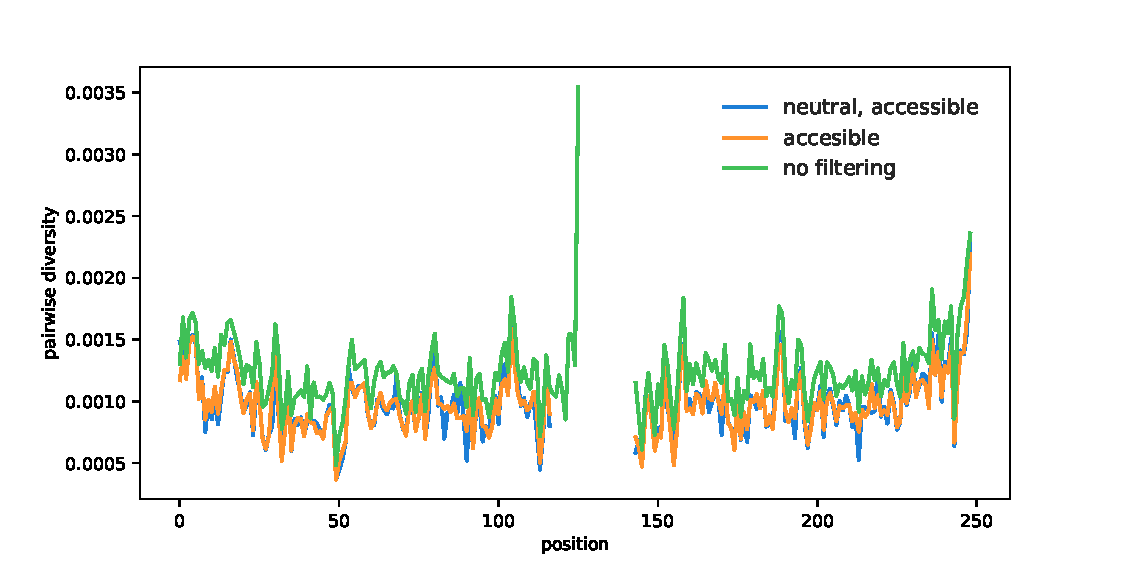
\includegraphics{figures/supplementary/chr1_diversity_filtering.pdf}

  \caption{Estimates of chromosome 1 YRI diversity in non-overlapping megabase
    windows, under different filtering criteria. The filtering criteria are,
    (1) ``neutral, accessible" which includes only putatively neutral sites, and
    ignores regions masked as inaccessible, (2) ``accessible" which is only ignores
  sites masked as inaccessible, and (3) ``no filtering" which uses all available
data. Note that filtering changes the absolute level of diversity, but has more
minor effects on regional patterns of diversity at the megabase scale.}

  \label{suppfig:chr1-diversity}
\end{figure}

\begin{table}
\centering
\begin{tabular}{lrrr}
  \hline
chrom &  accessible &  neutral &  both \\
  \hline
 chr1 &        42.4 &     64.4 &  22.9 \\
 chr2 &        46.8 &     58.7 &  23.7 \\
 chr3 &        44.1 &     62.9 &  24.8 \\
 chr4 &        44.0 &     59.3 &  21.5 \\
 chr5 &        44.1 &     58.0 &  21.4 \\
 chr6 &        45.0 &     58.0 &  22.1 \\
 chr7 &        44.4 &     65.8 &  26.4 \\
 chr8 &        43.8 &     61.2 &  23.1 \\
 chr9 &        39.2 &     64.5 &  20.3 \\
chr10 &        44.6 &     62.8 &  25.3 \\
chr11 &        42.7 &     63.5 &  23.4 \\
chr12 &        41.7 &     62.7 &  22.7 \\
chr13 &        39.7 &     62.0 &  18.3 \\
chr14 &        37.6 &     65.4 &  19.0 \\
chr15 &        37.0 &     69.4 &  20.3 \\
chr16 &        39.4 &     63.8 &  20.9 \\
chr17 &        40.4 &     64.0 &  22.3 \\
chr18 &        40.9 &     59.8 &  19.8 \\
chr19 &        30.9 &     69.8 &  18.0 \\
chr20 &        36.9 &     61.6 &  19.8 \\
chr21 &        31.6 &     68.6 &  18.2 \\
chr22 &        26.9 &     75.0 &  16.4 \\
\end{tabular}
\end{table}

\subsection{Estimates of Pairwise Diversity}

Our underlying data for all likelihood and pairwise diversity estimates is the
allele count matrix $\mathbf{C}$ with dimensions $L \times 2$, where $L$ is the
chromosome length. This is converted to a pairwise summary matrix with
identical dimensions, $\mathbf{P}$. The first column of $\mathbf{P}$ is the
number of pairwise comparisons between chromosomes that are identical, and the
second column is the number that are different. Both of these columns are
combinatoric summaries of the allele counts matrix. Let $[c_1, c_2]$ be a row
of $\mathbf{C}$ for basepair $l$, and $n = c_1 + c_2$. Then, the (1) total
number of pairwise combinations of chromosomes $n_T$, (2) the number of
pairwise with identical alleles $n_S$, and (3) the number of pairwise
combinations with differing alleles $n_D$ are respectively,

\begin{align*}
  n_T &= \frac{n(n-1)}{2} \\
  n_S &= {c_1 \choose 2} + {c_2 \choose 2} \\
  n_D &= n_T - n_S
\end{align*}

Thus $\mathbf{P}_l = [n_S, n_D]$, and the pairwise diversity across the $n$
sampled chromosomes is calculated as

\begin{align}
  \pi(l) = \frac{n_D}{n_T}
\end{align}

which is identical to the more common expression of this estimator, 

\begin{align}
  \pi(l) = \frac{2}{n(n-1)} \sum_{i < j}^n k_{i,j}
\end{align}

where $k_{i,j}$ is 1 if the alleles at this site differ, and 0 otherwise. Note
that for sites with missing data, $c_1 = c_2 = 0$ and thus $n_T = 0$ and the
division is invalid. Such cases were marked as missing with floating point
values \texttt{NaN}s. Binned summaries of data are weighed by the number of
complete cases, e.g. rows with $c_1 + c_2 > 0$.

This per-basepair diversity is then averaged over all callable bases, to give a
genome-wide or window estimate of diversity of accessible bases in the set
$\mathcal{A}$,

\begin{align*}
  \bar{\pi}(\mathcal{A}) = \frac{\sum_{l \in \mathcal{A}} \pi(l)}{L_\mathcal{A}}.
\end{align*}

where $L_\mathcal{A} = |\mathcal{A}|$ is the number of accessible bases. Note
that the sum in the numerator is random over the sample of chromosomes sampled
from the population. Estimates of pairwise diversity often condition on the
accessible bases, and thus treat this as fixed. However, the number of
accessible bases varies across the chromosome; this can lead to a source of
apparent bias during block-bootstrap estimates of uncertainty.  In this case,
pairwise diversity is a ratio estimator, and is thus biased, since by Jensen's
inequality $\E(\nicefrac{y}{x}) \ge \nicefrac{\E(y)}{\E(x)}$ for random
variables $x$ and $y$.

\subsection{Window-based Summaries and filtering}

\begin{figure}[!htb]
  \centering
  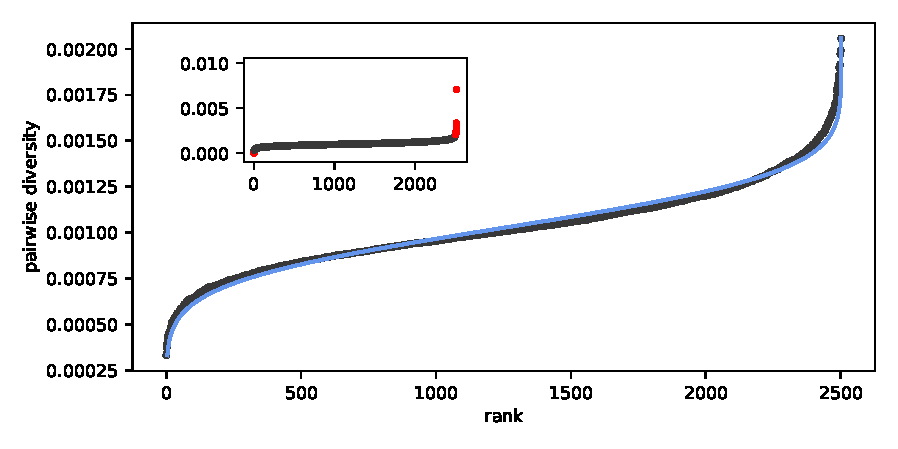
\includegraphics{figures/supplementary/diversity_trimming_dist.pdf}
  \caption{}
  \label{suppfig:trimming}
\end{figure}



The likelihood method is fit to non-overlapping binned summaries of the allele
counts matrix. 


Based on exploratory data analyses, some bins were outliers and
excluded (XXX).

\begin{enumerate}
  \item \textbf{Fraction of inaccessible sites per window}.  \path{mask_inaccessible_bins_frac}
  % \item \textbf{Edge truncation}

  \item \textbf{Outliers}: Based on exploratory analysis, there were some
    regions with very high diversity. The 0.05\% right tail was excluded.

\end{enumerate}


% supp data
% - npy files
% - edge trunation

  

\section{}

\printbibliography

\end{document}
